\chapter{Becoming (un)grammatical}

In the late 13th century, \textit{verray} (\textit{very}) began its journey in the English language. It was an adjective with a clear mission: to denote what was `true,' `real,' and `genuine.' Coming to English from the Anglo-French \textit{verrai}, it was rooted in the Latin \textit{verus}, meaning `true,' the source of words like \textit{verify}, \textit{verdict}, and \textit{warlock} (truly!).

When \textit{very} was getting its start, \textit{much} was already an English veteran, having survived several centuries and various incarnations. It likely started out in Proto-Germanic as something like \textit{mekilaz}  `great', related to words like \textit{majesty}, \textit{major}, and \textit{magnify}. But eventually, in Old English, it became \textit{micel}, meaning `great in size', as in (\ref{ex:micele-great}) from Genesis 1:16.

\ea\label{ex:micele-great}
  \gll \textit{God} \textit{geworhte} \textit{twá} \uline{\textit{micele}} \textit{leóht}.\\
       God created two \uline{great} lights .\\
  \trans `God made two great lights.'
\z

This use of \textit{much} is archaic, but it led to the Old- and Modern-English sense of `great in amount or extent', as in (\ref{ex:micele-much}).

\ea\label{ex:micele-much}
  \gll \textit{Oftor} \textit{micle}\\
       oftener much\\
  \trans `much more often'
\z

\textit{Verray} was going through its own development. The original meaning is still with us in expressions like \textit{the very heart of the matter}, but as the years rolled on, \textit{verray} explored new territories of meaning. By the late 14th century, it had expanded to signify `actual' and `sheer', gradually branching into a new role as an intensifier in the mid-15th century. This was a significant shift; \textit{verray} was stepping into the realm of adverbs.

In this new role, \textit{verray} began to encroach on the territory of \textit{much}. In 1481, a published text could say, 
\begin{quote}
    On they took their way: on the right side, they left Jaffa, and through a great plain and an even way, they came into the city of Lde, where the body of the glorious martyr Saint George lies. In his honor, Justinian, who was Emperor of Rome, made there a \uline{very fair} and rich church. But when the Turks heard news that our men were coming, they knocked it down and burned the timber work, which was \uline{very large}. They feared that our pilgrims would take them to make engines for casting stones and castles to assault with. Then our barons heard say that nearby was a \uline{very noble} city named Rames.
\end{quote}

\noindent Except that in Middle English, it was like this:
\begin{quote}
     \textit{on they toke their way: on the right side they lefte iaphe and by a grete playn and euen waye they cam in to the Cyte of lde where the bodye of the glorious martir seynt gorge lyeth: in thonoure of whom iustynyen that was Emperour of rome made there a \uline{moche fair} chirche and ryche but whan the turkes herde tydynges that our men cam they bete it doun and brence te tymbre werke whiche was \uline{moche grete} for they doubed that oure pilgrims shold take them for to make engyns to caste sons: and castellis to assaile with thenne herde our barons saye that ther fas by was a \uline{moche noble} Cyte named rames}\footnote{Caxton, William, 1481. Here begynneth the boke intituled Eracles, and also of Godefrey of Boloyne the whiche speketh of the conquest of the holy londe of Iherusalem ... \textit{Early English Books Online}.}
\end{quote}

Today, *\textit{much fair}, *\textit{much great}, and *\textit{much nobel} are ungrammatical. \textit{Much} can still modify adjectives, but it strongly prefers the comparative forms like \textit{much fairer}, \textit{much greater}, and \textit{much more nobel}, avoiding most plain-form adjectives; *\textit{much great} is no longer quite so great. \textit{Very} has developed complementary tendencies, such that it's happy modifying a plain-form adjective, as in \textit{very strange}, but modifying a comparative seems *\textit{very stranger}.

What might have happened, though, if \textit{very} hadn't appeared? Perhaps we would still be using *\textit{much great}. But appear it did, and from the 1470s until the 1530s, all it did, it seems, was to usurp more an more of \textit{much}'s turf. From the mid 1500s on, though, the use of \textit{much} started to recover as the two words specialized. In Modern English, both \textit{very} and \textit{much} are ubiquitous. Occurring roughly a thousand times per million words, \textit{very} is the 105th most frequent word in American English, with \textit{much} in 148th spot.\footnote{COCA} Still, like the poor child who makes good, or the team that comes from behind to win, \textit{very} had a hard row to hoe. 

\begin{figure}[ht]
    \centering
    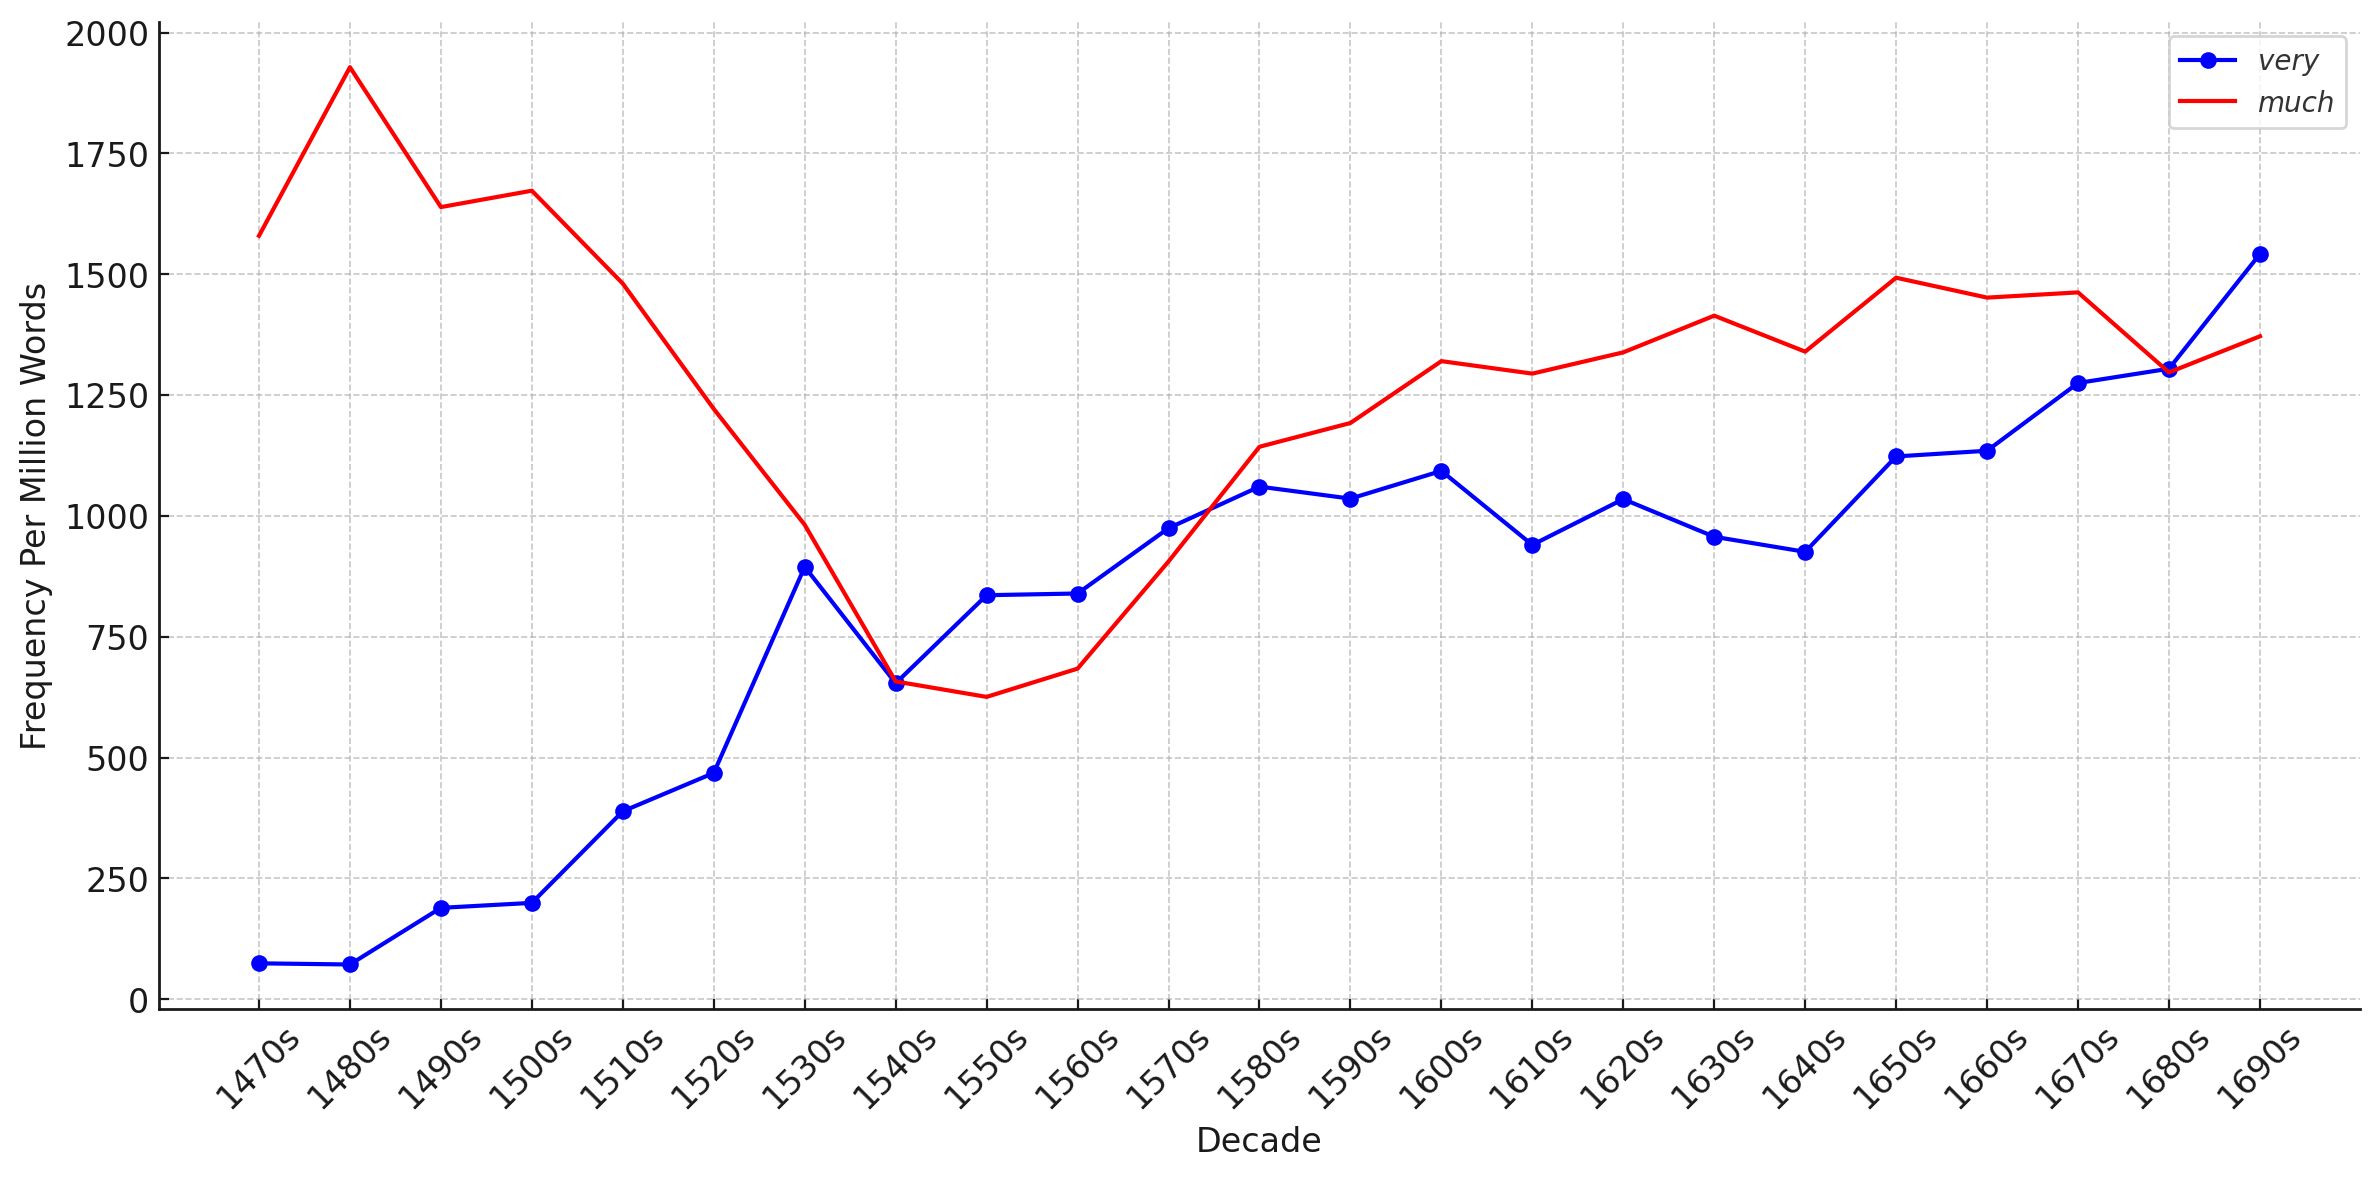
\includegraphics[width=\textwidth]{figures/very.png}
    \caption{The frequency of \textit{very} and \textit{much} (in various spellings) in the \textit{Early English Books Online} corpus, from the 1470s to the 1690s, shown per million words.}
    \label{fig:very-frequency}
\end{figure}

This is the story of \textit{much fair}'s journey from being perfectly normal in Middle English to *much ungrammatical today. But it's also a story about the very subtle and puzzling predilections that \textit{much} has accumulated over the last thousand years or so. How is it that we can say \textit{I don't know much about it}, but *\textit{I know much about it} is bad? And why is it saved when \textit{much} is modified by \textit{so} but not by \textit{very}? Why can \textit{much} almost never modify plain-form adverbs and yet \textit{much too \dots} is impeccable? How did all these \textit{much} constructions become ungrammatical?

\section{Pas de \textit{ne \dots~pas}}

In French, the negative has (or had) two parts: \textit{ne} and \textit{pas}, so that \textit{it doesn't work that way} would be \textit{Ça \uline{ne} marche \uline{pas} comme ça}. But it wasn't always so. In the early days of Old French, a simple placement of \textit{ne} before the verb was all that was required to negate a sentence. Its use was straightforward and unadorned. 

Today, though, *\textit{Ça \uline{ne} marche comme ça} is totally ungrammatical, and it's also a great example of the life-course of a grammatical construction. The development of the clausal negation in French, particularly the emergence and transformation of \textit{pas}, follow a pattern called Jespersen's Cycle. This cycle, conceptualized by the Danish linguist Otto Jespersen in 1917, outlines a three-stage progression in the treatment of negation within languages.

\begin{quote}
    The history of negative expressions in various languages makes us witness the following curious fluctuation: the original negative adverb is first weakened, then found insufficient and therefore strengthened, generally through some additional word, and this in its turn may be felt as the negative proper and may then in course of time be subject to the same development as the original word.
(Jespersen 1917: 4)
\end{quote}


The early days of Old French, when a simple \textit{ne} would do, represent the first stage of Jespersen's Cycle. As the centuries passed, though, the power of \textit{ne} to convey negation began to diminish. It was as if the speakers of French sought greater emphasis, a stronger affirmation of nothingness. This need for reinforcement led to the second stage of Jespersen's Cycle: the birth of double negation.

Words like \textit{rien} `nothing', \textit{point} `at all', \textit{personne} `nobody', and of course \textit{pas}, all of which had previously just intensified \textit{ne}, began to demand to be heard. Interestingly, these words originally had concrete, quotidian meanings: \textit{point} was `point', \textit{personne} meant \textit{person}, and \textit{pas} was literally `step'. The phrase \textit{Je ne marche pas} was akin to saying `I won't walk a step'.

By Middle French (14th to 17th centuries), \textit{ne} had weakened to the extent that its use as a ``single negative'' was becoming increasingly ungrammatical. As the language developed into Early Modern French (17th to 18th centuries), \textit{ne} continued to weaken, and folks began to drop it: \textit{Je ne march pas} had started to become \textit{Je marche pas}. The once-understudy \textit{pas} has stepped up to eclipse \textit{ne} in its role as the primary negator. This change marks the third and final stage of Jespersen's Cycle, where the original negator is overshadowed or even rendered obsolete.

A similar progression happens with slurs in what has been called the \textsc{euphemism treadmill}. A word like \textit{stupid} can start out as a non-judgemental description of someone in a stupor, but eventually becomes insulting. As it become a meaner word, a kinder alternative is sought, a word like \textit{retarded}, meaning simply slow. But as children get wind of this new use, they start using it to cruel and insulting purpose, and it too must be abandoned \citep{Taylor1974}. Although the euphemism treadmill pertains to the meaning of individual words and Jespersen's cycle to the grammatical system of negation, similar processes underlie both.

Jespersen's third stage is not yet complete for \textit{ne}, but it's well along in its trajectory. In the 20th and 21st centuries, the trend towards \textit{ne} dropping in everyday spoken French was increasingly prevalent, especially in informal contexts. It's observed across various dialects of French, including those spoken in France, Canada, and other Francophone regions. The formal rules of grammar laid down by the Académie Française still prescribe the use of \textit{ne} for negation, and these tend to be followed in written and formal spoken French, but it's often missing from everyday spoken language.

\begin{tcolorbox}[title=The normality of double negatives, colback=white, parbox] \label{sec:double-negs}
\setlength{\parindent}{1.5em}
    \noindent Despite their being stigmatized in Standard English, double negatives are actually quite common in the world's languages, to the extent that sometimes ``single negatives'' are out-and-out ungrammatical or impossible. For example, in Italian, the way to express `I never go' is \textit{non vado mai}, which more or less translates as `I don't never go.' *\textit{Vado mai} without \textit{non} ain't no good.
    
    The case of double negatives is a case where our sense of ungrammaticality may result from having been explicitly told that double negatives are both ungrammatical and illogical. (Illogical? Yeah, right!). 
\end{tcolorbox}


\subsection{Polarity items}

If \textit{pas} `step' seems like a strange way to intensify negation, consider the English expressions,  \textit{I was so tired that I couldn't move} and then think about how that changes when you add \textit{a muscle}. \textit{I couldn't move a muscle} seems like a more complete inability to move, ruling out not just major limb motion but even single muscle contractions. This is the sense in which \textit{pas} contributes to the negative meaning: it's not simply that I can't wander down to the shop -- I can't even put one foot in front of the other. The more \textit{pas} was used like this, the more it was bleached of its meaning, becoming something much closer to a pure negator.

\textit{A muscle}, in contrast, still has much of its basic meaning, but consider saying, \textsuperscript{?}\textit{I was so energized that I could move a muscle.} Grammatical, perhaps, but utterly bizarre. Other expressions of this sort are \textit{drink a drop}, \textit{sleep a wink}, \textit{lift a finger}, \textit{give a damn}, \textit{spend a red cent}, \textit{budge an inch}, \textit{bat an eyelash}, \textit{hold a candle to}, \textit{miss a beat}, \textit{show a spark of decency}, and \textit{hurt a fly} \citep[24]{Israel2011}.

\citet[3]{Israel2011} points out that

\begin{quote}
    these are not the sorts of facts one is likely to notice about a language, but they are remarkable nonetheless. One would expect that anything one could affirm, one could also deny, and that anything one could deny, one could also affirm. But polarity items are subject to special constraints, the violation of which results in unexpectedly unacceptable sentences.
\end{quote}

This brings us back to \textit{much}. In these constructions, \textit{pas} and \textit{a muscle} are what linguists call \textsc{negative polarity items} or NPIs for short, or \dots~\textsc{negatively-orientied polarity-sensitive items} for long \citep{cgel}. And so is \textit{much}. Among the most common phrases with \textit{much} are \textit{much time}, \textit{much money}, \textit{much fun}, \textit{much attention}, and \textit{much trouble}. But while you hear \textit{I~\uline{don't} really have \uline{much} time} all the time, nobody says, \textsuperscript{?}\textit{I~really have much time}.

At first blush, it seems odd that \textit{pas}, \textit{a muscle}, and \textit{much} would all be negative polarity items. A step or a muscle are the smallest possible ways to walk or move -- the next closest thing to not walking or moving -- which might explain their polarity preferences; being so energized that you can move a muscle is not being very energized at all. \textit{Much}, though, is all the way at the other end of the spectrum. It's great, majestic, magnitudinous, and magnificent. What might pull it down to negative levels?

\citet[82]{Israel2011} points out that degree modifiers like \textit{much} apply not just to positively oriented adjectives like \textit{bigger}, but also to negatively oriented ones like \textit{smaller}. If something is much smaller than something else, it

Consider, then a weak intensifier like \textit{pretty} as in \textit{that's pretty good}. If you're pretty smart, you're smart but hardly brilliant. A pretty good try is one with some effort behind it, but probably not enough to succeed. And telling your romantic interest that you love them pretty much is never a winning strategy. \textit{Pretty} is at the opposite end of the intensification scale to \textit{much}, and it's also a positive polarity item -- these things too exist -- at the opposite end of the polarity scale.



In 2023, I was writing a paper on \textit{much}, arguing that \textit{The Cambridge grammar of the English language} had made an error in saying it was sometimes an adverb, and I sent the paper to John Payne for comment. John had worked with Rodney Huddleston and Geoff Pullum on the book, and he was one of the listed authors on the chapter that made the claim about \textit{much}. As we went back and forth, looking at things from a variety of perspectives, John noticed something I hadn't, something perhaps nobody had before: \textit{much} is an NPI in many constructions (like \textit{not much time} or \textit{I don't drive much}) but not in adjective phrases like \textit{much bigger}. In other words, a positive assertion that \textit{it's much better} is just as good as the negative \textit{it's not much better}, while as we've seen \textit{I don't drive much} is much better than \textsuperscript{*}\textit{I drive much}.



And so I started looking at \textit{much}'s behaviour at different points in the past, trying to see if it had always been like that. I went the the \textit{Early English Books Online} corpus, and there, in a random sample of 100 uses of \textit{moche sorowe} `great sorrow' from the late 1400s and early 1500s, found only a single example was in a non-affirmative environment. A typical positive example would be (\ref{ex:moche-sorrow}).\footnote{1515. The cronycles of Englond. \textit{Early English books online}.}

\ea \label{ex:moche-sorrow}
    \gll \textit{his} \textit{peple} \textit{for} \textit{hym} \textit{made} \textit{moche} \textit{sorowe}. \\ his people for him made great sorrow.\\
    \trans `His people caused him great sorrow.'
\z

Now, you would certainly be correct to observe that such a situation doesn't sound particularly positive, but it's not negative in the sense that linguists have in mind when they speak about NPIs. Even in 1680, the last year of the corpus, only 16\% of the occurrences of \textit{much time} are in non-affirmative environments, certainly not what you would expect of an NPI. I switched then to the \textit{Corpus of Historical American English}, which starts 140 years later, in 1820. In that decade, only 8\% of my sample was in a non-affirmative environment. By the 1830s, 15\% were, 28\% in the 1840s, 27\% in the 1850s, and 31\% in the 1850s. Clearly, it was in the first half of the 19th century that \textit{much} became an NPI.

Unfortunately, I have no idea why that happened then, but it suggests that people developed a sense that \textit{much} was better in non-affirmative environments, without developing the feeling that it was ungrammatical there. Like a path in a forest that becomes more defined and specialized as more people walk it, \textit{much} in non-affirmative contexts became more specialized simply through the natural progression of language use. These kinds of changes tend to happen the way one goes bankrupt, according to Hemingway, slowly and then suddenly. It's like the ``S-shaped curve'' in Figure \ref{fig:sigmoid-function}.

\begin{figure}
    \centering
        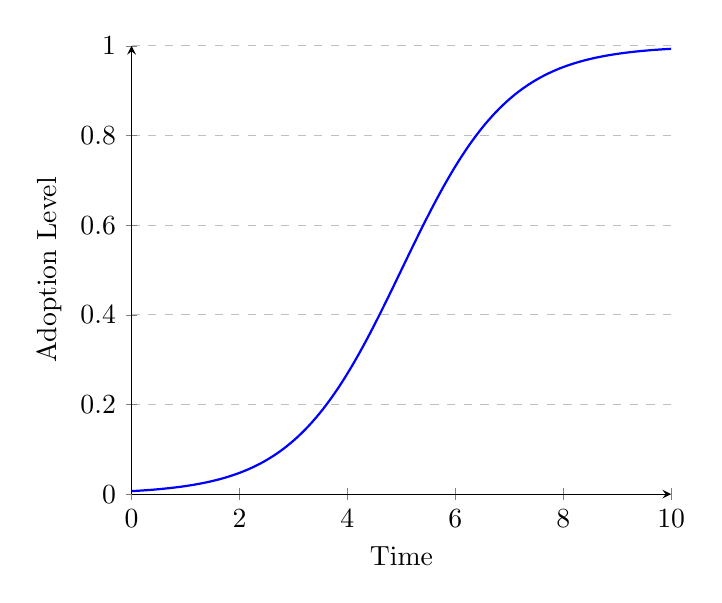
\begin{tikzpicture}
        \begin{axis}[
            xlabel={Time},
            ylabel={Adoption Level},
            xmin=0, xmax=10,
            ymin=0, ymax=1,
            axis lines=left,
            xtick={0,2,4,6,8,10},
            ytick={0,0.2,0.4,0.6,0.8,1},
            ymajorgrids=true,
            grid style=dashed,
        ]
        
        \addplot[
            domain=0:10,
            samples=100,
            smooth,
            thick,
            blue,
        ] {1/(1+exp(-1*(x-5)))};
        \end{axis}
        \end{tikzpicture}
    \caption{The typical adoption curve of language change.}
    \label{fig:sigmoid-function}
\end{figure}

But we can say something else about how these develop because very similar NPIs develop in very different languages. This is not some kind of structural similarity that might point to a ``universal grammar'' but rather semantic similarities that point to a role for semantics in understanding grammaticality.

\begin{quote}
    As the founder of modern linguistics, Saussure (1916)
pointed out, in all languages we find both centripetal and
centrifugal tendencies. The need to communicate creates
the centripetal force of linguistic homogenisation, which is
balanced by a centrifugal force of differentiation, driven by
an impetus for local identity, by the need to exchange
information without having the people from the next village
or the other religious community overhear, by the desire of
each new generation to mark itself off from the one before. \cite{Joseph2015}
\end{quote}

\section{Words}

``There dwelled Abram in wealth and in frith.'' This is translated from Middle English, keeping only the Middle English word \textit{frith} meaning `peace'. How does it register with modern readers given that its use is not ungrammatical, but the word is entirely unfamiliar?

\section{Assertion and presupposition}

A new sound, word, or construction comes into being by being used. One person simply \textsc{presupposes} that it will be understood by others, and, generally, it is, after which it can be taken as common knowledge. Even if it isn't fully clear, often we accommodate such innovations. In other words, it is establish just by being used.

In this way, it's like a declaration of marriage, money, promises and apologies, or a pass code on a debit card. 

\begin{quote}
In short, the continual attempt, by each of us, to determine our language's nature is the force that shapes it over time. Everyone acts as if the rules are already common knowledge, and then -- the strangest part! -- they gradually try to work out what this common knowledge is. This is strikingly different to determining the position of a planet, or the weight of a large cake, where there is a fact of the matter totally separate from our beliefs about it, which can be reconstructed by investigation through telescopes or scales. \hfill\citep{CohnGordon2024}
\end{quote}

\bigskip

But we don't accommodate just anything. 

Infants are born with an ability to distinguish between different accents. As you might expect, that ability isn't purely theoretical. By five or six months old, infants show a preference for people who speak with their native accent, and five-year-olds are more likely to want to be friends with children who have the same accent as theirs. This preference exists even if they can fully understand children with different accents \citep{Kinzler2007}. As they age, this kind of bias remains. For example, children are more likely to trust and learn from adults who speak with a similar accent to their own. This is demonstrated by their tendency to believe demonstrations of how to use new objects when those demonstrations are performed by adults with familiar accents \citep{Kinzler2011a}.

And there's every reason to believe that's how it goes with grammar too. When a child hears an unfamiliar construction from an adult who shares their native language, they should be likely to look for a motivation for that construction on. When they've heard it only from a non-native speaker, they're very likely to understand it, but they should also be very likely to see it as an error rather than as an innovation.

``This ‘how-possibly’ story for the evolution of vagueness is particularly interesting given previous game theoretic results due to Lipman [2009] indicating that, generally, vagueness is inefficient in common-interest signaling situations. The implication is that, while vagueness itself may not be evolutionarily benefi- cial, it may nonetheless persist in language because learning strategies that are themselves evolutionarily beneficial lead to vagueness'' \citep[708]{OConnor2014}.
